\documentclass[8pt,landscape]{article}
\usepackage[a4paper,top=0.5cm,bottom=0.5cm,left=0.5cm,right=0.5cm]{geometry}

\usepackage[ngerman]{babel}
\usepackage{graphicx}
\usepackage[utf8]{inputenc}
\usepackage{amsfonts}
\usepackage{multicol}
\setlength\parindent{0ex}
\usepackage{amsmath, amsfonts, amssymb}
\setlength{\columnsep}{10mm}
\usepackage{blindtext}
\usepackage{paralist}
\usepackage{bbm} % Natural numbers etc.
\usepackage[boxed]{algorithm2e}

\newcommand{\vmspace}{\vspace{-7pt}}
\newcommand{\vpspace}{\vspace{9pt}}


% -------------- Beginning of Document ---------------.
\begin{document}


\renewcommand{\labelitemi}{--}
%\setlist{noitemsep}
\pagestyle{empty}
\raggedright
\setlength{\columnsep}{2mm}
\setlength{\columnseprule}{0.1mm}
\begin{multicols}{3}
\title{\textbf{Autonomous\\ Mobile Robots}}
\author{Fabian Blöchliger}
\date{Spring Semester 2016}
\maketitle


\section{Introduction and Motivation}

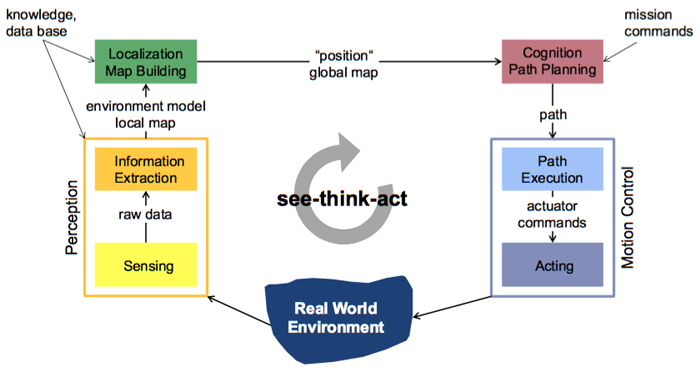
\includegraphics[width=\columnwidth]{img/1_SeeThinkAct.png}

\section{Locomotion Concepts}

\begin{minipage}{\columnwidth}
  To get from the inertial frame $I$ to body frame $B$:
  \begin{compactitem}
    \item \textbf{translate} with vector ${}_I\mathbf{r}_{OB}$,
    \item \textbf{rotate} with matrix $\mathbf{R}_{IB}$.
  \end{compactitem}
\end{minipage}

\vpspace

\begin{minipage}{\columnwidth}
  Express point $P$ which is given w.r.t frame $B$ in frame $I$:
  \vmspace
  \begin{center}
  ${}_I\mathbf{r}_{OP} = {}_I\mathbf{r}_{OB} +
  \mathbf{R}_{IB}\;{}_B\mathbf{r}_{BP}$.
  \end{center}
\end{minipage}

\vpspace

\begin{minipage}{\columnwidth}
  Equivalent \textbf{homogeneous transformation} description:
  \vmspace
  \begin{center}
    $\left(\begin{matrix}
      {}_I\mathbf{r}_{OP} \\
      1
    \end{matrix}\right)
    =
    \left(\begin{matrix}
      \mathbf{R}_{IB} & {}_I\mathbf{r}_{OB} \\
      0 & 1
    \end{matrix}\right)
    \left(\begin{matrix}
      {}_B\mathbf{r}_{BP} \\
      1
    \end{matrix}\right)$
  \end{center}
\end{minipage}

\vpspace

\begin{minipage}{\columnwidth}
  \textbf{Velocity} of rigid body point $P$:
  \vmspace
  \begin{center}
    ${}_I \mathbf v_P = {}_I \mathbf{\dot r}_{OP} = \mathbf{\dot r}_{OB} +
    {}_I\mathbf{\omega}_{IB} \times {}_I\mathbf r_{BP}.$
  \end{center}
\end{minipage}

\vpspace

\begin{minipage}{\columnwidth}
  \textbf{Differentiation} of moving frame vector:
  \vmspace
  \begin{center}
    ${}_B\mathbf v_P = {}_B\left(\mathbf{\dot r}_{OP}\right) = \dfrac{\mathrm
    d\, {}_B\mathbf r_{OP}}{\mathrm d \,t} + {}_B\omega_{IB} \times {}_B\mathbf
    r_{OP}$
  \end{center}
\end{minipage}

\vpspace

\begin{minipage}{\columnwidth}
  Basic rotation matrices $\mathbf R_x(\bullet)$, $\mathbf R_y(\bullet)$, $\mathbf
  R_z(\bullet)$:
  \vmspace
  \begin{center}
    $\left(\begin{matrix}
      1 & 0 & 0 \\
      0 & \cos & -\sin \\
      0 & \sin & \cos
    \end{matrix}\right),\;
    \left(\begin{matrix}
      \cos & 0 & \sin \\
      0 & 1 & 0 \\
      -\sin & 0 & \cos
    \end{matrix}\right),\;
    \left(\begin{matrix}
      \cos & -\sin & 0 \\
      \sin & \cos & 0 \\
      0 & 0 & 1
    \end{matrix}\right).$
  \end{center}
\end{minipage}

\vpspace

\begin{minipage}{\columnwidth}
  \textbf{Jacobian} (partial derivative of position vector $\mathbf{r}_{OP}$
  w.r.t. \textbf{generalized coordinate} vector $\mathbf{q}$):
  \vmspace
  \begin{center}
    $J_P = \dfrac{\partial \mathbf{r}_{OP}(\mathbf q)}{\partial \mathbf q}$.
  \end{center}
\end{minipage}

\vpspace

\begin{minipage}{\columnwidth}
  Left/right pseudoinverse for $m \times n$ matrix $\mathbf{J}$ to solve
  $\mathbf r_F = \mathbf J_F \mathbf q$ for $\mathbf q$:
  \vmspace
  \begin{center}
    $\mathbf{J}^+=
    \begin{cases}
      (\mathbf{J}^\intercal \mathbf J)^{-1} \mathbf J^\intercal, & m>n\;\;
      \text{(overdetermined)},\\
      \mathbf J^\intercal (\mathbf{J} \mathbf J^\intercal)^{-1}, & m<n\;\;
      \text{(underdetermined).}
    \end{cases}$
  \end{center}
\end{minipage}

\vpspace

\begin{minipage}{\columnwidth}
  Iterative approach for \textbf{inverse kinematics} of robotic manipulator to
  find generalized coordinates for end-effector position $\mathbf r^\text{goal}$
  (Newton's method):\\
  \vmspace
  \begin{algorithm}[H]
    $\mathbf q = \mathbf q^0$\;
    $\mathbf r = \mathbf r(\mathbf q)$\;
    \While{$\| \mathbf r - \mathbf r^\mathrm{goal} \| > \mathrm{threshold}$}
    {
    $\mathbf q = \mathbf q + \mathbf J^+(\mathbf q) \cdot (\mathbf r^\text{goal}
    - \mathbf r)$\;
    $\mathbf r = \mathbf r ( \mathbf q )$\;
    }
    \Return $\mathbf q$.
  \end{algorithm}
\end{minipage}

\vpspace

\begin{minipage}{\columnwidth}
  Inverse \textbf{differential kinematics} (get desired end-effector velocity
  $\mathbf{\dot{r}_F}$):
  \vmspace
  \begin{center}
    $\mathbf{\dot r}_F = \mathbf J_F \mathbf{\dot q}$
    $\;\;\rightarrow\;\;$
    $\mathbf{\dot q} = \mathbf J_F^+ \mathbf r_F.$
  \end{center}
\end{minipage}

% TODO
% - Check column-rank / row-rank deficiency.

\section{Mobile Robot Kinematics}

\blindtext[3]

\section{Perception I}

\blindtext[3]

\section{Perception II}

\blindtext[3]

\section{Perception III}

\blindtext[3]

\section{Perception IV}

\blindtext[3]

\section{Localization I}

\blindtext[3]

\section{Localization II}

\blindtext[3]

\section{SLAM I}

\blindtext[3]

\section{SLAM II}

\blindtext[3]

\section{Planning I}

\blindtext[3]

\section{Planning II}

\blindtext[3]





\end{multicols}

% -------------- End of Document ---------------------. 
\end{document}
